% コンパイル: lualatex paper_ja.tex
\documentclass[10pt,twocolumn]{ltjsarticle}
\usepackage{luatexja-fontspec}
\setmainjfont{IPAexMincho}
\setsansjfont{IPAexGothic}
\usepackage[a4paper,margin=18mm]{geometry}
\usepackage{graphicx}
\usepackage{amsmath}
\usepackage{amssymb}
\usepackage{booktabs}
\usepackage{enumitem}
\usepackage[hidelinks]{hyperref}

\setlength{\columnsep}{6mm}

\begin{document}

\twocolumn[{%
  \begin{center}
    {\LARGE\bfseries 33Bオムニモーダル動画生成モデルへのキャラクタLoRA微調整}\\
    \vspace{0.6em}
    {\large ——律速要因はVRAMではなくシステムRAMであった——}\\
    \vspace{1.2em}
    {\large Masato Suzuki (Masafy)}\\
    \vspace{0.4em}
    {2026年8月15日}
  \end{center}
  \vspace{1.0em}
  {\centering\textbf{要 旨}\par}
  \vspace{0.4em}
  \begingroup\small
  \noindent 本報告は、著者の先行研究——Stable Diffusion~1.5（約10億パラメータ）~\cite{suzuki2026sd15lora} および Krea~2（約120億パラメータ）~\cite{suzuki2026krea2lora} に対するキャラクタLoRA微調整——を、動画生成の領域へ拡張する試みである。対象は映像と音声を同時に生成するオムニモーダルモデル \textbf{MiniMax~H3}（拡散トランスフォーマ約330億パラメータ、テキストエンコーダに Qwen3-VL~320億パラメータを併用）であり、先行研究と同一の被写体（著者が個人制作したレッサーパンダキャラクター「マサフィー」）を用いた。先行2研究はいずれも VRAM~12\,GB の消費者向けGPU 1台で学習が成立することを示したが、\textbf{本研究では同一のGPUで学習が成立しなかった}。その原因を実測により追跡した結果、律速要因は VRAM ではなく\textbf{システムRAM}であることが判明した。学習時の VRAM 実測ピークは 3{,}959\,MiB（使用したGPU搭載量の2.8\%）に留まる一方、モデル群41.2\,GB の読み込み過程でシステムRAM~50\,GB の環境では OOM により3回失敗し、188\,GB の環境で初めて完走した。さらに (a) 学習済みLoRAは量子化形式を跨いで移植可能（枝刈りINT8 で学習し GGUF~Q3\_K\_M で推論、208モジュール全一致）であり推論は VRAM~9.3\,GB で完結すること、(b) 参照画像方式を用いる場合の LoRA の寄与は構造的安定性ではなく\emph{画風}にあること、(c) 適用強度は画風の忠実性と構造の正確性のトレードオフを構成し、学習段階と強度の交差検証により推奨設定が 500ステップ・強度0.8 と定まること、を実験的に示した。一連の作業に要した計算費用は約5米ドルである。

  \par\medskip
  \noindent\textbf{キーワード:}\ 動画生成, オムニモーダルモデル, 拡散トランスフォーマ, 低ランク適応, LoRA, システムメモリ, 量子化, 消費者向けGPU, 再現性
  \endgroup
  \vspace{2.0em}
}]

\section{はじめに}

著者は先行研究において、個人制作のオリジナルキャラクター「マサフィー」を、Stable Diffusion~1.5~\cite{suzuki2026sd15lora} および Krea~2~\cite{suzuki2026krea2lora} へ低ランク適応（LoRA）~\cite{hu2022lora} で追加学習し、いずれも VRAM~12\,GB の消費者向けGPU 1台で実用的な生成が可能であることを示した。特に後者では、120億パラメータのモデルに対し FP8 量子化とブロックスワップを併用することで、半精度なら重みだけで約24\,GBを要する規模の学習を12\,GBに収めた。

これら2つの成功は「\emph{適切な工夫により、消費者向けGPU 1台で最新モデルの個人向け微調整は成立する}」という一般的な主張を支持するものであった。本研究は、この主張が\textbf{動画生成モデル}に対しても成立するかを検証する。

対象とする MiniMax~H3 は、映像と音声を同時に生成するオムニモーダルモデルであり、拡散トランスフォーマ部が約330億パラメータ、テキストエンコーダとして Qwen3-VL の320億パラメータ版を併用する。参照画像からキャラクタを固定する Reference-to-Video-Audio（以下 R2V）の機能を持つ。

研究設問は以下の3点である。

\begin{itemize}[leftmargin=2.2em,topsep=2pt,itemsep=1pt]
  \item[\textbf{Q1.}] 先行研究と同一の VRAM~12\,GB のGPUで、330億パラメータ級の動画生成モデルへの LoRA 学習は成立するか。成立しない場合、真の制約は何か。
  \item[\textbf{Q2.}] 学習した LoRA は、学習時と異なる量子化形式の推論環境へ移植できるか。推論に要する資源はどの程度か。
  \item[\textbf{Q3.}] 参照画像でキャラクタを固定できる方式において、LoRA は何を寄与するのか。最適な適用強度と学習段階はどこか。
\end{itemize}

\textbf{本研究の主要な貢献は、Q1に対する否定的な回答と、その原因の同定にある。} 先行2研究が積み上げた主張の限界を、著者自身が定量的に示すものである。

\section{対象と方法}

\subsection{モデルの構成}

対象モデルの構成を表~\ref{tab:model} に示す。注目すべきはテキストエンコーダが320億パラメータである点で、本体と合わせ実質的に650億パラメータ級のモデル群を読み込むことになる。この事実が後述する制約の直接の原因となった。

\begin{table}[t]
\centering\small
\caption{対象モデルの構成}
\label{tab:model}
\begin{tabular}{lr}
\toprule
構成要素 & サイズ \\
\midrule
Transformer（枝刈りINT8 ConvRot） & 20.0\,GB \\
Text Encoder（Qwen3-VL 32B） & 15.7\,GB \\
VAE（映像 fp16 / 音声 fp32） & 5.5\,GB \\
\midrule
合計 & 41.2\,GB \\
\bottomrule
\end{tabular}
\end{table}

\subsection{学習設定}

学習には ai-toolkit~\cite{aitoolkit2026}（commit \texttt{f4e9130} に固定）を用いた。LoRA は rank~16 / alpha~16、対象モジュールは \texttt{attn.qkv\_proj}、\texttt{attn.out\_proj}、\texttt{mlp.fc1}、\texttt{mlp.fc2} であり、50ブロックと token\_refiner を合わせて\textbf{208モジュール}（416テンソル）に適用される。

データセットは著者が制作したキャラクタ画像 1000$\times$1000 を学習12枚・検証2枚・除外2枚とした。フレーム数は1（静止画を1フレーム動画として扱う）、バッチサイズ1、勾配チェックポイント有効、精度 bf16、解像度は512および768である。

キャプションは全画像が \texttt{masafy\_character,} で始まり、続けて外見の特徴（飛行帽ゴーグル、模様入りスカーフ）を記述し、最後にポーズ・表情・背景を画像ごとに記述する構造とした。\texttt{caption\_dropout\_rate} は 0.05 である。

\begin{figure*}[t]
\centering
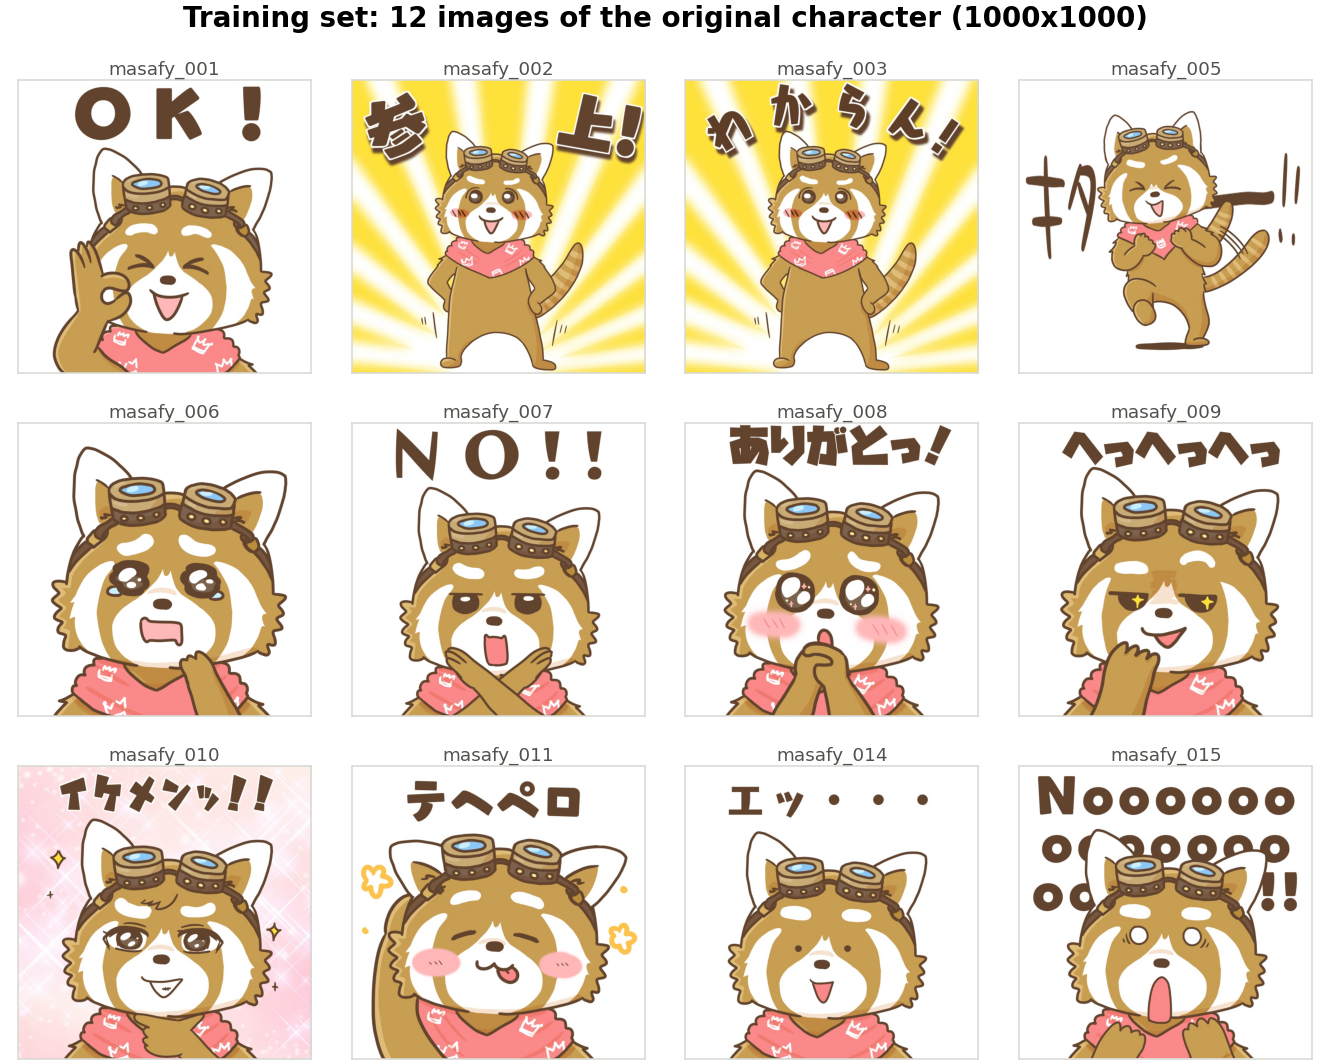
\includegraphics[width=\linewidth]{figures/fig_dataset.png}
\caption{学習データ。著者が制作したキャラクタ画像12枚。ステッカー用途のため、多くが切り抜き用の縁取りを含む。}
\label{fig:dataset}
\end{figure*}

\subsection{実行環境}

比較のため4種の環境で試行した（表~\ref{tab:env}）。VRAM とシステムRAM の双方を記録している点が本研究の要点である。

\begin{table*}[t]
\centering\small
\caption{実行環境と結果。VRAM は成否を予測しないが、システムRAM は予測する。}
\label{tab:env}
\begin{tabular}{llrrrl}
\toprule
環境 & GPU & VRAM & システムRAM & 単価 & 結果 \\
\midrule
ローカル & RTX 3060 & 12\,GB & 30\,GB & 電気代のみ & 失敗（2時間25分で0ステップ） \\
クラウドA & A40 & 48\,GB & 50\,GB & \$0.44/h & 失敗（OOM, \texttt{low\_vram}有効） \\
クラウドA' & A40 & 48\,GB & 50\,GB & \$0.44/h & 失敗（OOM, \texttt{low\_vram}無効） \\
クラウドB & H200 SXM & 141\,GB & 233\,GB & \$4.59/h & 成功（予備実験） \\
クラウドC & RTX 6000 Ada & 48\,GB & 188\,GB & \$0.84/h & 成功（本学習） \\
\bottomrule
\end{tabular}
\end{table*}

\section{Q1：律速要因の同定}

\subsection{ローカル環境での失敗}

先行研究と同一の RTX 3060（VRAM~12\,GB / RAM~30\,GB）で予備学習を試みたところ、\textbf{2時間25分の経過に対し完了ステップ数は0}であった。GPU使用率は全観測点で0.0\%であり、\texttt{Quantizing transformer} の直後で停止、生成物は得られなかった。

GPU使用率が終始0\%であったことは、GPUが計算を待たされていたのではなく\emph{計算に到達する前段で詰まっていた}ことを示す。\texttt{low\_vram} オプションによりCPU側へ重みを退避する設定であったが、モデル群41.2\,GB に対しシステムRAMは30\,GBであり、スワップ領域への退避が発生していたと考えられる。

ここから得られる第一の教訓は、\textbf{\texttt{low\_vram} 系のオプションが存在することは動作可能性を意味しない}という点である。VRAMだけでなく、モデル全体を保持できるシステムRAMの有無を先に確認する必要がある。

\subsection{クラウド環境での再現と切り分け}

VRAM~48\,GB / RAM~50\,GB の環境で本学習を試みたところ、いずれも同一地点で強制終了した（終了コード137, SIGKILL）。

\begin{quote}\small\ttfamily
Loading Qwen3-VL text encoder\\
 - attached 351 pre-quantized layers\\
Text encoder is already quantized\\
Killed
\end{quote}

Transformer 20.0\,GB の読み込み後、テキストエンコーダ 15.7\,GB を積んだ時点で36\,GBに達し、実行環境のオーバーヘッドを加えて上限50\,GBを突破したと考えられる。

重要な観察として、\texttt{low\_vram} を無効化した2回目の試行でも\textbf{同じ地点で失敗した}。これは重みの読み込みが「一旦システムRAMへ展開してからGPUへ転送する」経路を通るためであり、VRAMの空き容量とは独立に失敗することを意味する。事実、この時点でのVRAM使用量は 0--3\,MiB であった。

RAM~188\,GB および 233\,GB の環境では、いずれも問題なく完走した。したがって本モデルの学習に必要なシステムRAMは\textbf{50\,GB超・188\,GB以下}の範囲にある。

図~\ref{fig:constraint} に、環境ごとの VRAM・システムRAM と成否の対応を示す。VRAM は48\,GBの環境で失敗も成功も起きており成否を予測しないが、システムRAM は50\,GBと188\,GBの間に明確な閾値を持つ。

\begin{figure*}[t]
\centering
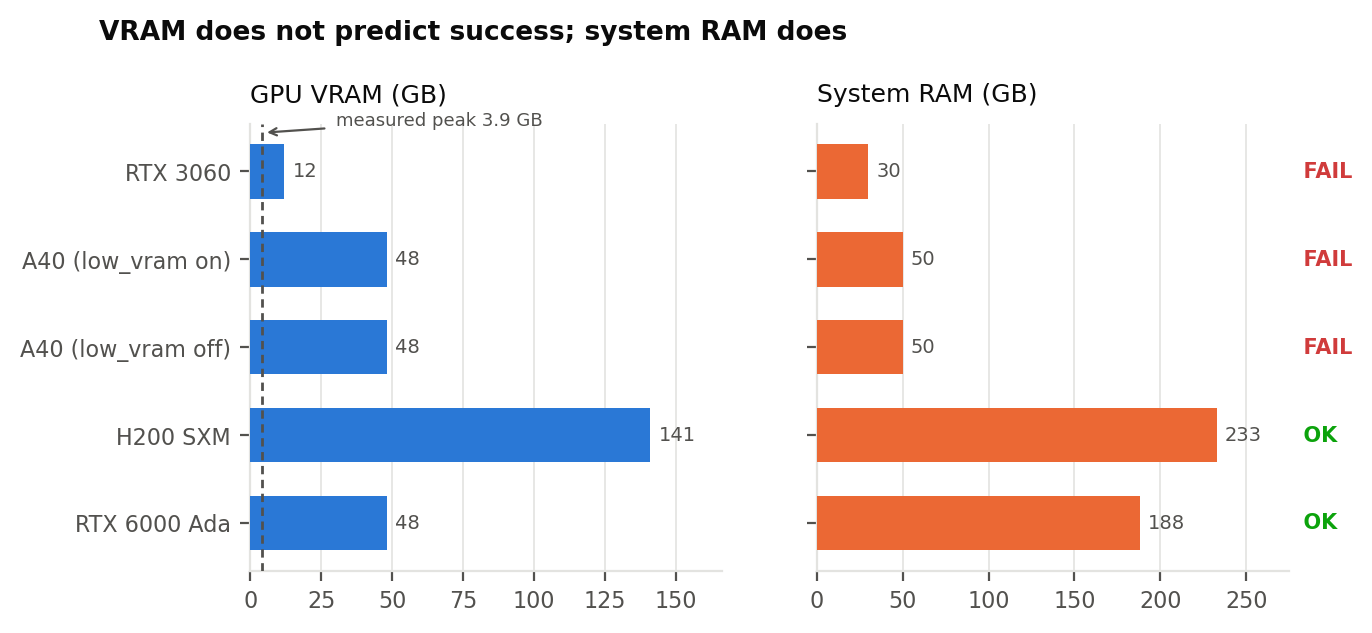
\includegraphics[width=\linewidth]{figures/fig_constraint.png}
\caption{VRAM は成否を予測せず、システムRAM が予測する。破線は学習時のVRAM実測ピーク（3.9\,GB）。}
\label{fig:constraint}
\end{figure*}

\subsection{提供環境のRAM割当は価格と相関しない}

商用クラウドの提供構成を調査した結果、システムRAMの割当がGPUの価格帯ともVRAM容量とも相関しないことが判明した（表~\ref{tab:ram}）。

\begin{table}[t]
\centering\small
\caption{提供構成のRAM割当（公表値）}
\label{tab:ram}
\begin{tabular}{lrrr}
\toprule
GPU & VRAM & システムRAM & 単価 \\
\midrule
RTX 3090 & 24\,GB & 125\,GB & \$0.50/h \\
RTX 4090 & 24\,GB & \textbf{41\,GB} & \$0.69/h \\
RTX 6000 Ada & 48\,GB & 167\,GB & \$0.84/h \\
A40 & 48\,GB & \textbf{50\,GB} & \$0.44/h \\
H100 NVL & 94\,GB & \textbf{94\,GB} & \$3.19/h \\
\bottomrule
\end{tabular}
\end{table}

RTX 4090 は RTX 3090 より高価でありながらRAMは3分の1である。当初計画では4090を用いる予定であったが在庫の都合で確保できなかった。\emph{仮に確保できていた場合、A40 より早い段階で失敗していた}ことになる。

さらに、同一GPU型番であっても提供形態により割当が異なる。第三者がホストする形態の RTX 3090 を確保したところ、実測RAMは 30\,GB および 41\,GB であり、公表値の125\,GBとは大きく異なった（独立試行は2回）。

\subsection{本学習の実測値}

RTX 6000 Ada（RAM~188\,GB, \$0.84/h）で800ステップの学習を実行した。1ステップあたり 9.04秒（最終ステップまで安定）、総経過 2時間00分15秒、費用 \$1.89 であった。損失の推移を図~\ref{fig:loss} に示す。

\begin{figure}[t]
\centering
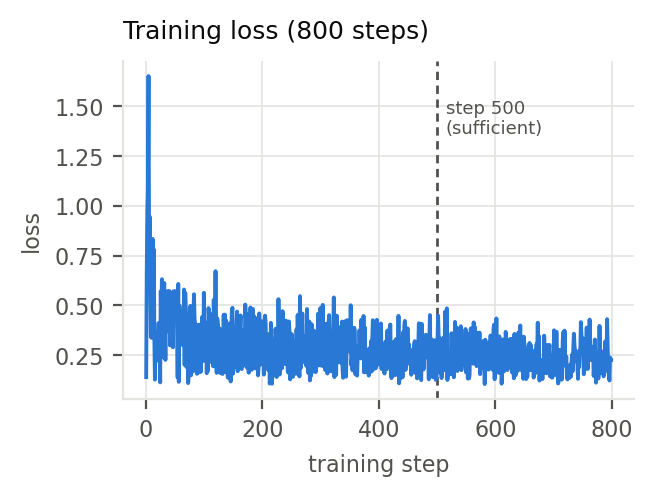
\includegraphics[width=\linewidth]{figures/fig_loss.png}
\caption{学習の損失推移（800ステップ、799点を記録）。}
\label{fig:loss}
\end{figure}

なお環境構築時間はvCPU数に強く依存した。vCPU~9 の環境では2{,}100秒を要したが、vCPU~14--24 の環境では147--366秒であった。\textbf{高価なGPUほど付随するvCPUも多く初期構築も速い}ため、「高価な環境では準備時間の固定費が不利になる」という当初の予想は成立しなかった。

\subsection{付随して観察された障害}

パッケージマネージャが既定で導入する PyTorch は CUDA~13 向けビルドであったが、実行環境のドライバは CUDA~12.8 までの対応であった。この状態でも学習プロセスは正常に起動し進捗も報告し続けるが、実体はCPU上で動作しており計算が進まない（\texttt{torch.cuda.is\_available()} が偽）。

対処として \texttt{torch==2.13.0+cu126} を明示指定して再導入した。ここで\textbf{バージョン番号のみを指定した再導入は無効である}。既に同一バージョン番号が導入されているため、パッケージマネージャはビルドタグの差異を認識せず何も実行しない。ローカルバージョン識別子まで含めた指定を要する。

この障害は「動作しているが計算が進まない」形で顕在化し、第3.1節の症状と外形的に区別できない。したがって、\textbf{学習開始前に \texttt{torch.cuda.is\_available()} を検査し、偽であれば開始しない}検査を導入すべきである。

\section{Q2：量子化を跨いだ移植}

学習は枝刈りINT8形式の safetensors に対して行われた一方、推論環境は GGUF~Q3\_K\_M 形式を使用する。両者は同一モデルの異なる量子化であり、重みキーが一致する保証はない。

推論環境へ適用したところ、\texttt{208 patches attached} と報告され、これは LoRA が対象とする 50ブロック$\times$4モジュール + token\_refiner と完全に一致した。キー不一致の警告は0件であった。

\textbf{量子化形式が異なっても、レイヤー名の構造が保たれていれば LoRA は移植可能である。} これは学習と推論で異なる量子化を選択できることを意味し、実務上の自由度は大きい。

推論時のVRAM使用量は 9{,}326\,MiB であり、生成時間は 864$\times$480・5秒の動画に対し RTX 3060 で約13分であった。\textbf{学習には188\,GBのシステムRAMを備えた環境が必要であったが、推論は手元の消費者向けGPUで完結する。} この非対称性は本研究の実用的な含意である。

\section{Q3：LoRAの寄与と最適設定}

\subsection{LoRAは何を寄与するのか}

R2V は参照画像によりキャラクタを固定する方式である。したがって「参照画像で固定できるのであれば LoRA は不要ではないか」という疑問が生じる。この問いに答えるため、\textbf{LoRAの有無のみを変えた対照実験}を行った。参照画像には検証用データセットの1枚（学習に使用していない画像）を用い、プロンプト・乱数種・解像度・サンプリングステップ数は同一に固定した。

結果は表~\ref{tab:ablation} の通りである。LoRA非適用でも、参照画像によってキャラクタは破綻せず描出され、装飾品も正しく描かれ、フレーム間のちらつきも生じない。\textbf{しかし画風が全く異なるものとなる。}

\begin{table}[t]
\centering\small
\caption{LoRAの有無による差（同一条件）}
\label{tab:ablation}
\begin{tabular}{lll}
\toprule
評価項目 & 適用 & 非適用 \\
\midrule
構造的安定性 & 良好 & 良好 \\
ちらつき & なし & なし \\
装飾品の描出 & 良好 & 良好 \\
\textbf{画風の忠実性} & \textbf{良好} & \textbf{全く異なる} \\
出力サイズ & 525\,KB & 1{,}087\,KB \\
\bottomrule
\end{tabular}
\end{table}

\begin{figure*}[t]
\centering
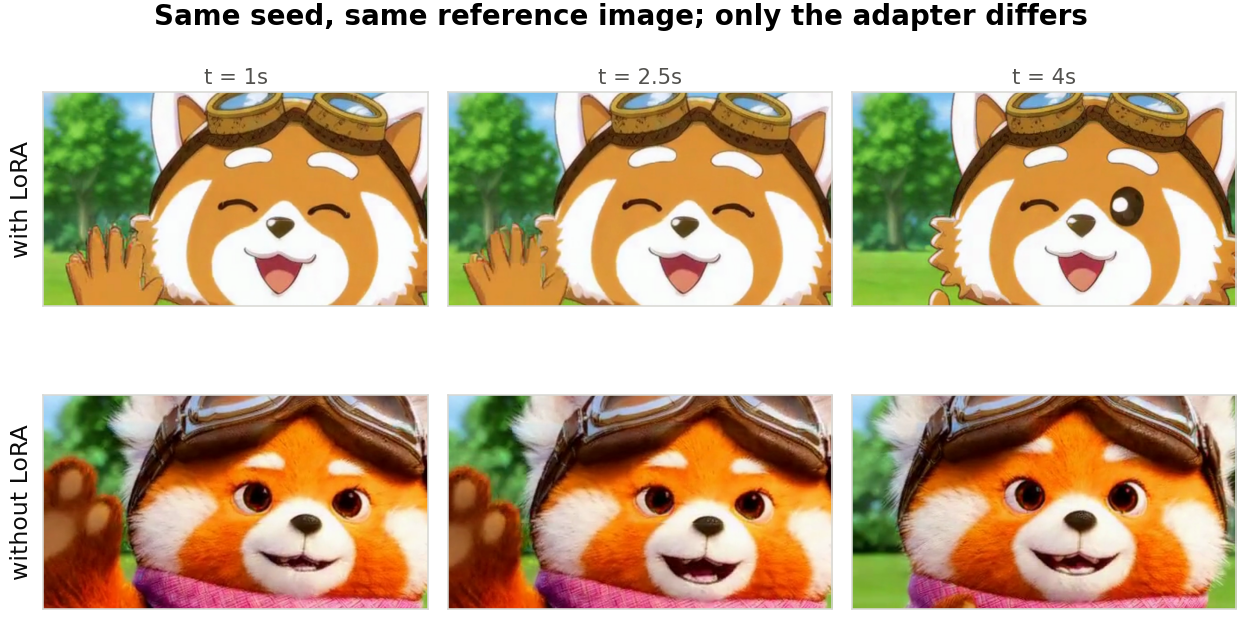
\includegraphics[width=\linewidth]{figures/fig_ablation_frames.png}
\caption{同一seed・同一参照画像で、アダプタの有無のみを変えた生成結果。上段は平坦な塗りのイラスト、下段は毛並みまで描かれた写実的な描画となる。}
\label{fig:abframes}
\end{figure*}

したがって役割は次のように分離される。\emph{参照画像は「何が描かれるか」を伝達し、LoRA は「どう描かれるか」を担う。} 「参照画像で固定できるなら LoRA は不要」という推論は誤りであり、キャラクタLoRAの投資対効果は「キャラクタを出せるようになること」ではなく\textbf{自分の画風で出せるようになること}にある。

\subsection{適用強度と学習段階}

適用強度（0.0--1.2）および学習段階（300--800ステップ）を変化させた計24本の動画を、他の条件を固定して生成し定性評価を行った（図~\ref{fig:strength}, 図~\ref{fig:checkpoint}）。

\begin{figure}[t]
\centering
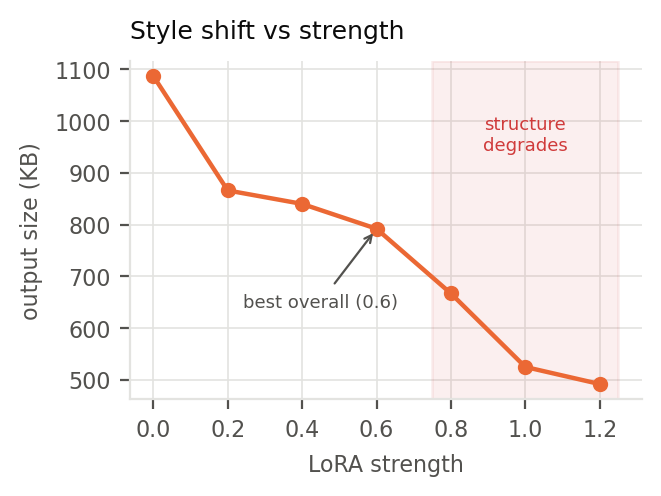
\includegraphics[width=\linewidth]{figures/fig_strength.png}
\caption{適用強度と画風の移行。出力サイズは画風の移行度の代理指標。}
\label{fig:strength}
\end{figure}

\begin{figure}[t]
\centering
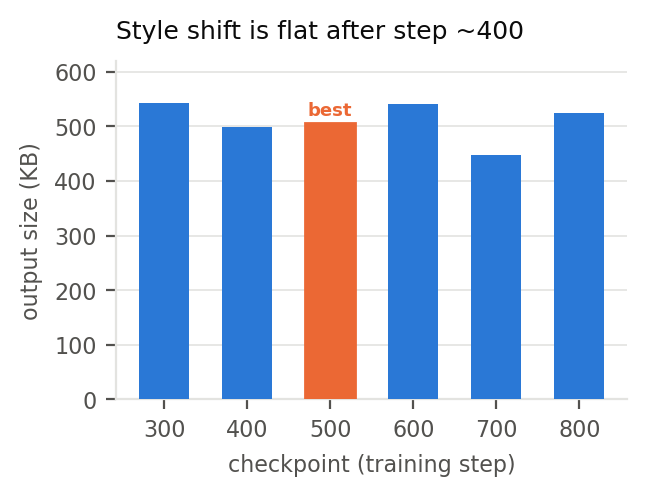
\includegraphics[width=\linewidth]{figures/fig_checkpoint.png}
\caption{学習段階による差。400ステップ以降は画風の移行が頭打ちになる。}
\label{fig:checkpoint}
\end{figure}

\textbf{画風の忠実性と構造の正確性はトレードオフの関係にある。} 強度を上げるほど画風は目標に近づくが、手など複雑な部位の描出が破綻する。また学習段階については、500ステップ付近で画風の獲得が完了しており、それ以降の学習は改善に寄与していない。むしろ700ステップでは軽微な破綻が観察された。

\subsection{交差検証と推奨設定}

上記2つの比較は、強度については800ステップ版で、学習段階については強度1.0で実施したため、それぞれの最良値の組み合わせが未検証であった。そこで学習段階500ステップにおいて強度 0.6 / 0.8 / 1.2 を追加生成し、交差検証を行った。

結果、\textbf{500ステップ・強度0.8 が総合的に最良}であった。強度0.6では画風の移行が不十分であり、強度1.2では画風は最も目標に近いものの、\emph{キャラクタ全体を太い暗色の輪郭線が囲む}現象が現れた。これは学習データがステッカー用途の切り抜き画像であったことに由来する特徴の再現であり、静止画では自然でも動画中では違和感を生じる。

\begin{figure*}[t]
\centering
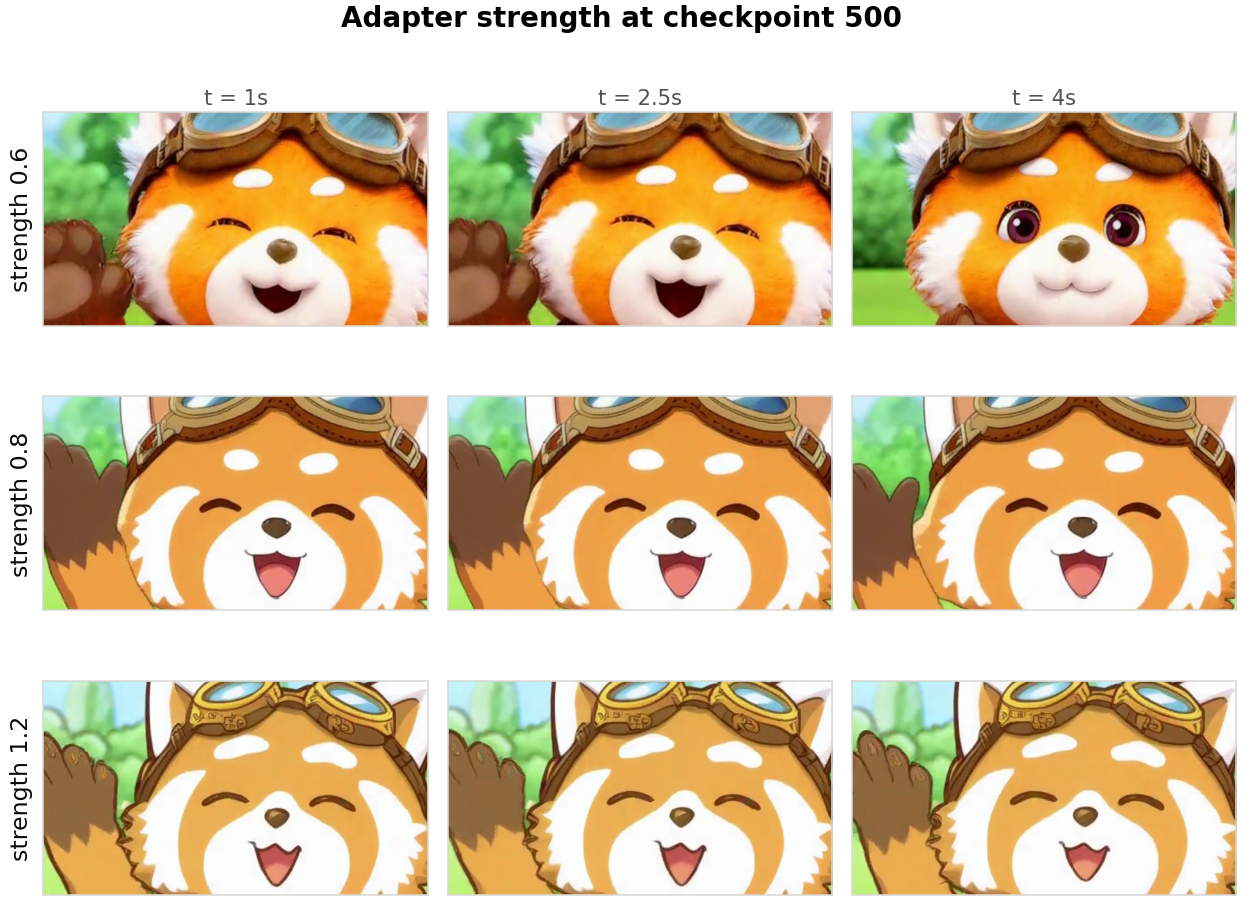
\includegraphics[width=\linewidth]{figures/fig_strength_frames.png}
\caption{学習段階500における適用強度の比較。強度1.2ではキャラクタ全体を太い暗色の輪郭線が囲む。}
\label{fig:stframes}
\end{figure*}

したがって推奨設定は\textbf{500ステップ・強度0.8}であり、当初採用した800ステップ・強度1.0は\emph{学習・推論の双方において過剰}であった。学習時間は約2時間から約1.25時間へ、費用は \$1.89 から約 \$1.2 へ削減できたことになる。

\subsection{データセット設計が持ち込むもの}

交差検証の過程で、LoRAが学習データの性質を予期せぬ形で持ち込むことが観察された。

第一に、前述の\textbf{輪郭線}である。ステッカー画像に含まれる切り抜き用の縁取りが、強度を上げると再現される。

第二に、\textbf{細部の再現には強度を要する}点である。キャプションに \texttt{pink patterned scarf} と記述されているにもかかわらず、強度0.6および0.8ではスカーフはほぼ無地であり、模様が現れるのは強度1.2である。

第三に、\textbf{LoRAは背景にも作用する}。強度0.6では被写界深度のある背景であったものが、強度1.2では記号的な描線となる。キャプションが画像全体を説明する形式であったためであり、「キャラクタのみを差し替える」用途には効果が広すぎる。

これらはいずれも、\emph{キャプション設計とデータセットの性質が、そのまま出力の性質として現れる}ことを示している。

\subsection{トリガー語の有効性}

トリガー語を除去して外見記述のみを与えた場合、各要素は描出されるものの画風が失われた。トリガー語のみを与え外見記述を省いた場合、生成は成立しなかった。すなわち\textbf{LoRAは外見情報を完全には内包しておらず、キャプション中の外見記述が実質的な役割を担っている}。学習データが12枚と少なく、かつ全キャプションに外見記述を含めた設計に起因すると考えられる。

\subsection{出力サイズという代理指標}

出力ファイルサイズは画風の移行度と単調な相関を示した（強度0.0の1{,}087\,KBから強度1.2の492\,KBまで単調減少）。学習データが平坦な塗りのイラストであるため、画風が目標に近づくほど階調が減少し動画コーデックの圧縮効率が向上するためと考えられる。

ただし\textbf{サイズは品質の指標としては機能しない}。最小値を示した強度1.2および700ステップの出力は、いずれも構造的な破綻あるいは違和感を含んでいた。サイズが測定しているのは画風の移行度のみである。

\section{限界}

\begin{enumerate}[leftmargin=1.6em,topsep=2pt,itemsep=2pt]
  \item \textbf{学習時のシステムRAMピーク使用量を実測できていない。} 監視機構がGPU統計のみを記録しており、システムRAMの記録項目を欠いていた。したがって要件は「50\,GBでは不足、188\,GBでは十分」という範囲としてしか示せない。後続の測定のため計測機構を実装済みである。
  \item \textbf{費用は概算である。} A40 での試行を開始する前の残高を測定していないため、総額は約5米ドルとしか言えない。API により実測できた区間は \$3.44 である。
  \item \textbf{定性評価は単一の評価者による主観評価である。} 複数評価者による盲検評価は行っていない。
  \item \textbf{データセットは12枚と小規模}であり、トリガー語の有効性および汎化能力に関する結論は、この規模に固有の可能性がある。
  \item \textbf{未学習場面への汎化は限定的}であった。学習データに存在しない場面（夜間の街路、自転車走行）では、LoRA適用時にディテールの破綻が観察された。
\end{enumerate}

\section{結論}

330億パラメータのオムニモーダル動画生成モデルへの LoRA 学習において、律速要因は VRAM ではなく\textbf{システムRAM}であった（Q1）。学習時の VRAM 実測ピークは 3{,}959\,MiB（搭載量の2.8\%）に留まる一方、システムRAM~50\,GB の環境では読み込み段階で失敗し、188\,GB の環境で完走した。

先行研究~\cite{suzuki2026sd15lora,suzuki2026krea2lora} が示した「消費者向けGPU 1台で成立する」という主張は、本研究の対象規模では\textbf{成立しない}。ただしその理由は、当初想定された「VRAMが足りない」ではなく「システムRAMが足りない」であった。したがって同種の学習において借用すべきは「VRAMの大きいGPU」ではなく\textbf{システムRAMの大きい計算機}である。提供されるRAM容量はGPUの価格帯ともVRAM容量とも相関しないため、意識的な確認を要する。

学習済み LoRA は量子化形式を跨いで移植可能であり、推論は VRAM~9.3\,GB で完結する（Q2）。\textbf{学習のみを外部環境に委託し、運用を手元の消費者向けGPUで行う構成が成立する}。

参照画像方式を用いる場合、LoRA の寄与は構造的安定性ではなく画風の再現にある（Q3）。適用強度は画風の忠実性と構造の正確性のトレードオフを構成し、交差検証の結果、推奨設定は\textbf{500ステップ・強度0.8}である。当初採用した設定は過剰であった。

一連の作業に要した計算費用は約5米ドルである。

\section*{再現性}

学習・検証に用いたスクリプト、データセット、実測ログ、および本稿の原稿は以下で公開している。

\begin{itemize}[leftmargin=1.4em,topsep=2pt,itemsep=0pt]
\item \url{https://github.com/masafykun/minimax-h3-masafy-lora}
\item \url{https://huggingface.co/masafy/minimax-h3-masafy-lora}
\end{itemize}

\begin{thebibliography}{9}
\bibitem{suzuki2026sd15lora} M.~Suzuki. 個人制作キャラクターの画像生成LoRAファインチューニング——消費者向けGPUを用いた少数データ条件下での実験的検討——. 技術報告, 2026.
\bibitem{suzuki2026krea2lora} M.~Suzuki. 12Bパラメータ画像生成モデルへのキャラクタLoRA微調整——消費者向け単一GPU上でのFP8量子化とブロックスワップ、および蒸留モデルへの転移——. 技術報告, 2026. DOI: 10.5281/zenodo.20838898.
\bibitem{hu2022lora} E.~J.~Hu, Y.~Shen, P.~Wallis, Z.~Allen-Zhu, Y.~Li, S.~Wang, L.~Wang, and W.~Chen. LoRA: Low-Rank Adaptation of Large Language Models. \textit{International Conference on Learning Representations (ICLR)}, 2022.
\bibitem{peebles2023dit} W.~Peebles and S.~Xie. Scalable Diffusion Models with Transformers. \textit{IEEE/CVF International Conference on Computer Vision (ICCV)}, 2023.
\bibitem{lipman2023flowmatching} Y.~Lipman, R.~T.~Q. Chen, H.~Ben-Hamu, M.~Nickel, and M.~Le. Flow Matching for Generative Modeling. \textit{International Conference on Learning Representations (ICLR)}, 2023.
\bibitem{ruiz2023dreambooth} N.~Ruiz, Y.~Li, V.~Jampani, Y.~Pritch, M.~Rubinstein, and K.~Aberman. DreamBooth: Fine Tuning Text-to-Image Diffusion Models for Subject-Driven Generation. \textit{IEEE/CVF Conference on Computer Vision and Pattern Recognition (CVPR)}, 2023.
\bibitem{qwenimage2025} Qwen Team. Qwen-Image Technical Report. 2025.
\bibitem{aitoolkit2026} ostris. AI Toolkit. \url{https://github.com/ostris/ai-toolkit}, 2026.
\bibitem{comfyui2026} comfyanonymous. ComfyUI. \url{https://github.com/comfyanonymous/ComfyUI}, 2026.
\end{thebibliography}

\end{document}
